\documentclass[11pt, a4paper]{article}

\usepackage[utf8]{inputenc}
\usepackage[a4paper, total={6in, 8in}]{geometry}
\raggedbottom

\usepackage{mlmodern}
\usepackage{csquotes}
\usepackage{parskip}
\usepackage[italian]{babel}
\usepackage{booktabs}
\usepackage{multicol}
\usepackage{graphicx}
\usepackage{fancyhdr}
\usepackage{float}
\usepackage{changepage}
\usepackage{fancyvrb}
\usepackage[final]{pdfpages}
\usepackage{placeins}
\usepackage{hyperref}
\usepackage[all]{hypcap}
\usepackage{tcolorbox}
\usepackage{xurl}
\usepackage{xcolor}
\usepackage{tikz}
\usepackage{biblatex}
\usepackage{array}
\usepackage{pdfpages}
\usepackage{subfig}
\usepackage{multirow}
\usepackage{pgfplots}
\usepackage{listings}
\usepackage{subfig}
\usepackage{caption}
\usepackage{pdfpages}
\usepackage{placeins}
\usepgfplotslibrary{groupplots}
\pgfplotsset{compat=1.17}


\addbibresource{bibliography.bib}

\hypersetup{
	colorlinks=false,
	citecolor=black,
	filecolor=black,
	linkcolor=black,
	urlcolor=black,
	allbordercolors=white
}


\definecolor{codegreen}{rgb}{0,0.6,0}
\definecolor{codegray}{rgb}{0.5,0.5,0.5}
\definecolor{codepurple}{rgb}{0.58,0,0.82}
\definecolor{backcolour}{rgb}{0.95,0.95,0.92}

\lstdefinestyle{mystyle}{
	backgroundcolor=\color{backcolour},   
	commentstyle=\color{codegreen},
	numberstyle=\tiny\color{codegray},
	stringstyle=\color{codepurple},
	basicstyle=\ttfamily\footnotesize,
	breakatwhitespace=false,         
	breaklines=true,                 
	captionpos=b,                    
	keepspaces=true,                   
	numbersep=5pt,                  
	showspaces=false,                
	showstringspaces=false,
	showtabs=true,                  
	tabsize=1
}

\lstset{style=mystyle}

\setlength{\headheight}{14pt}

\begin{document}
	\begin{center}
	{\LARGE \textbf{Università degli Studi di Milano Bicocca}} \\
	\vspace{0.2cm}
	{\Large {Dipartimento di Informatica}} \\ 
	\vspace{1cm}
	
	
\includegraphics[width=4cm]{figures/unimib-logo.png} \\
	\vspace{0.4cm}
	
	{\huge \textbf{Metodi del calcolo scientifico}} \\ 
	\Large{Compressione di immagini attraverso la DCT}
	\vspace{3cm}
\end{center}
\vspace{2cm}

\noindent \large{Membri del gruppo:} 

\begin{tabular}{@{}lll}
	\textbf{Canesi Gabriele} & 851637 & \href{mailto:g.canesi1@campus.unimib.it}{\texttt{g.canesi1@campus.unimib.it}}\\
	\textbf{Fiorenza Gioele} & 851631 & \href{mailto:g.fiorenza1@campus.unimib.it}{\texttt{g.fiorenza1@campus.unimib.it}}\\
	\textbf{Ghislotti Gianluca} & 859242 & \href{mailto:g.ghislotti@campus.unimib.it}{\texttt{g.ghislotti@campus.unimib.it}}\\
\end{tabular}

\vfill
\begin{center}
	\large{\textbf{Anno Accademico 2022/2023}}
\end{center}




	\thispagestyle{empty}
	\newpage
	\pagestyle{fancy}
	\pagenumbering{roman}
	
	
	\tableofcontents
	
	\newpage
	
	\definecolor{fireenginered}{rgb}{0.81, 0.09, 0.13}
	\hypersetup{
		linkbordercolor=fireenginered
	}
	\pagenumbering{arabic}
	
		
\part{Implementazione della DCT2}

Lo scopo di questa parte del progetto è stato quello di implementare la nostra versione della DCT2 e confrontare i tempi di esecuzione con quelli di una libreria che implementa la versione fast della DCT2. La libreria utilizzata è la FFTW \cite{fftw}, scritta in C.

Per testare la scalatura eseguita da FFTW, applichiamo una dct e una idct su una matrice di partenza per poi testare se tali valori corrispondono tra loro. Dalla differenza dei risultati ottenuti, abbiamo osservato che viene introdotto un errore durante le operazioni non superiore ad 1e$^{-14}$. Consideriamo tale errore di approssimazione accettabile, osservando che la differenza tra 2 double successivi è pari a 2.22045e$^{-16}$.

L'implementazione "fatta in casa" della DCT2 e dell'analoga IDCT2 è stata implementata tramite la sua versione ad una singola dimensione, infatti una 2-D discrete cosine transform è semplicemente una doppia applicazione della versione ad una dimensione. Così facendo, abbiamo codificato la cosine transform ad una singola dimensione, per poi chiamarla sia sulle righe che sulle colonne, ottenendo in questo modo una 2-D cosine transform.

\section{Informazioni sulla libreria}

La libreria scelta, come accennato precedentemente, è la FFTw, il cui nome è l'abbreviativo di \textit{Fast Fourier Transform in the West}. Infatti si dichiara essere una delle implementazioni più veloci della Fastest Fourier Transform. Tali risultati sono stati raggiunti grazie ad un ottimizzazione particolare degli algoritmi, che sfruttano alcune istruzioni specifiche dei vari processori ottimizzate per la risoluzione numerica.

L'implementazione effettiva risale al '97, nonostante ciò gode di particolare popolarità su Github\cite{Github} e ha vinto numerosi premi, tra cui il \textit{1999 J.H Wilkinson Prize for Numerical Software}, il quale viene conferito, una volta sola ogni 4 anni, al software che "best addresses all phases of the preparation of high quality numerical software", ovvero al programma che meglio copre tutte le fasi di un software numerico. Inoltre il paper correlato alla libreria "A Fast Fourier Transform Compiler"\cite{fftw_paper} ha ricevuto il premio di "Most Influential PLDI Paper" nel 2009, con un totale di circa 2000 download e 400 citazioni.

\section{Implementazione custom}

Il codice implementato per eseguire la DCT, secondo la definizione de coefficienti vista a lezione, è il seguente:


\begin{lstlisting}[gobble=1]
	void dct(int N, double *in, double *out, int jump = 1) {
		
		double *f = new double[N];
		
		for (int i = 0; i < N; ++i) {
			f[i] = in[i * jump];
		}
		
		for (int i = 0; i < N; ++i) {
			
			double a_i = 0;
			
			for (int j = 0; j < N; ++j) {
				a_i +=  f[j] * cos(i * M_PI * (2 * j + 1) / (2 * N));
			}
			
			a_i /= (i == 0 ? N : N/2);
			out[i * jump] = a_i;
		}
		
		delete[] f;
	}

\end{lstlisting}

Siccome l'applicazione di 2 dct genera la DCT2, di seguito si trova la sua implementazione:

\begin{lstlisting}[gobble=1]
	void dct2(int N, int M, double *in, double *out) {
		for (int i = 0; i < N * M; ++i) {
			out[i] = 0;
		}
		
		// Rows
		for (int i = 0; i < N; ++i) {
			dct(M, in + i * M, out + i * M, 1);
		}
		
		// Columns
		for (int i = 0; i < M; ++i) {
			dct(N, out + i, out + i, M);
		}
	}
\end{lstlisting}

Il codice della DCT prende in input il puntatore alla matrice di output per fare in modo che la DCT2 possa eseguire due DCT in place, ovvero scrivendo due volte sulla stessa matrice evitando ulteriori allocazioni di memoria.

Per evitare il calcolo del prodotto scalare delle basi con sè stesse, inoltre, abbiamo controllato direttamente l'indice della frequenza: se questo è 0, allora il prodotto scalare sarà N, altrimenti corrisponderà sempre a $\frac{N}{2}$.

Inoltre, è presente un parametro \textit{jump}, che fa in modo che la DCT salti di un certo numero di celle di memoria per passare da una componente alla successiva: la sua utilità si concretizza nel momento in cui viene chiamata la DCT sulle colonne: la matrice è organizzata in modalità row major, per cui, per eseguire la dct in place sulle colonne, è necessario dire alla DCT di saltare di M celle per passare alla componente successiva del vettore "logico", dove M rappresenta il numero di colonne della matrice.

\section{Test}

All'interno del codice sono stati aggiunti una serie di test (tramite l'uso delle assert) all'interno dei quali viene verificato l'esito dell'applicazione della DCT e della IDCT sulla matrice e sul vettore fornito. Successivamente l'esecuzione del codice prosegue verificando i tempi e generando un csv contenente i risultati delle esecuzioni su matrici man mano sempre più grandi. Dai risultati presenti nell'immagine \ref{fig:timings}, si può osservare come l'implementazione "fatta in casa" (in figura denominata \textit{Slow}) abbia effettivamente un andamento più esponenziale rispetto la liberia (in figura \textit{Fast}). Un fenomeno particolare che si osserva è che mentre la matrice è ancora di dimensioni molto ristrette la dct implementata fatta da noi supera quella fast. Una possibile ragione è che la FFTW utilizza delle tecniche numeriche sulla trasformata per ridurre il numero di operazioni necessarie, il che porta ad una maggiore efficienza per matrici di elevate dimensioni. Analogamente, nelle matrici di piccole dimensioni, è ragionevole pensare che l'applicazione di queste tecniche introducano un overhead che porta ad avere una performance peggiore rispetto alla DCT2 standard.

FFTW non esegue lo stesso algoritmo ad ogni chiamata della DCT: questo è il motivo per cui il grafico della versione fast non è liscio come quello della versione "fatta in casa", che esegue sempre lo stesso tipo di istruzioni indipendentemente dalla matrice/vettore in input.
È importante puntualizzare inoltre che, anche se questo non influisce sui tempi, i risultati delle DCT e DCT2 sono diversi tra la versione fast e la nostra: infatti, la libreria presa in considerazione utilizza un tipo di scaling della matrice dei coefficienti diverso da quello visto a lezione.

\begin{figure}[ht]
	\centering
	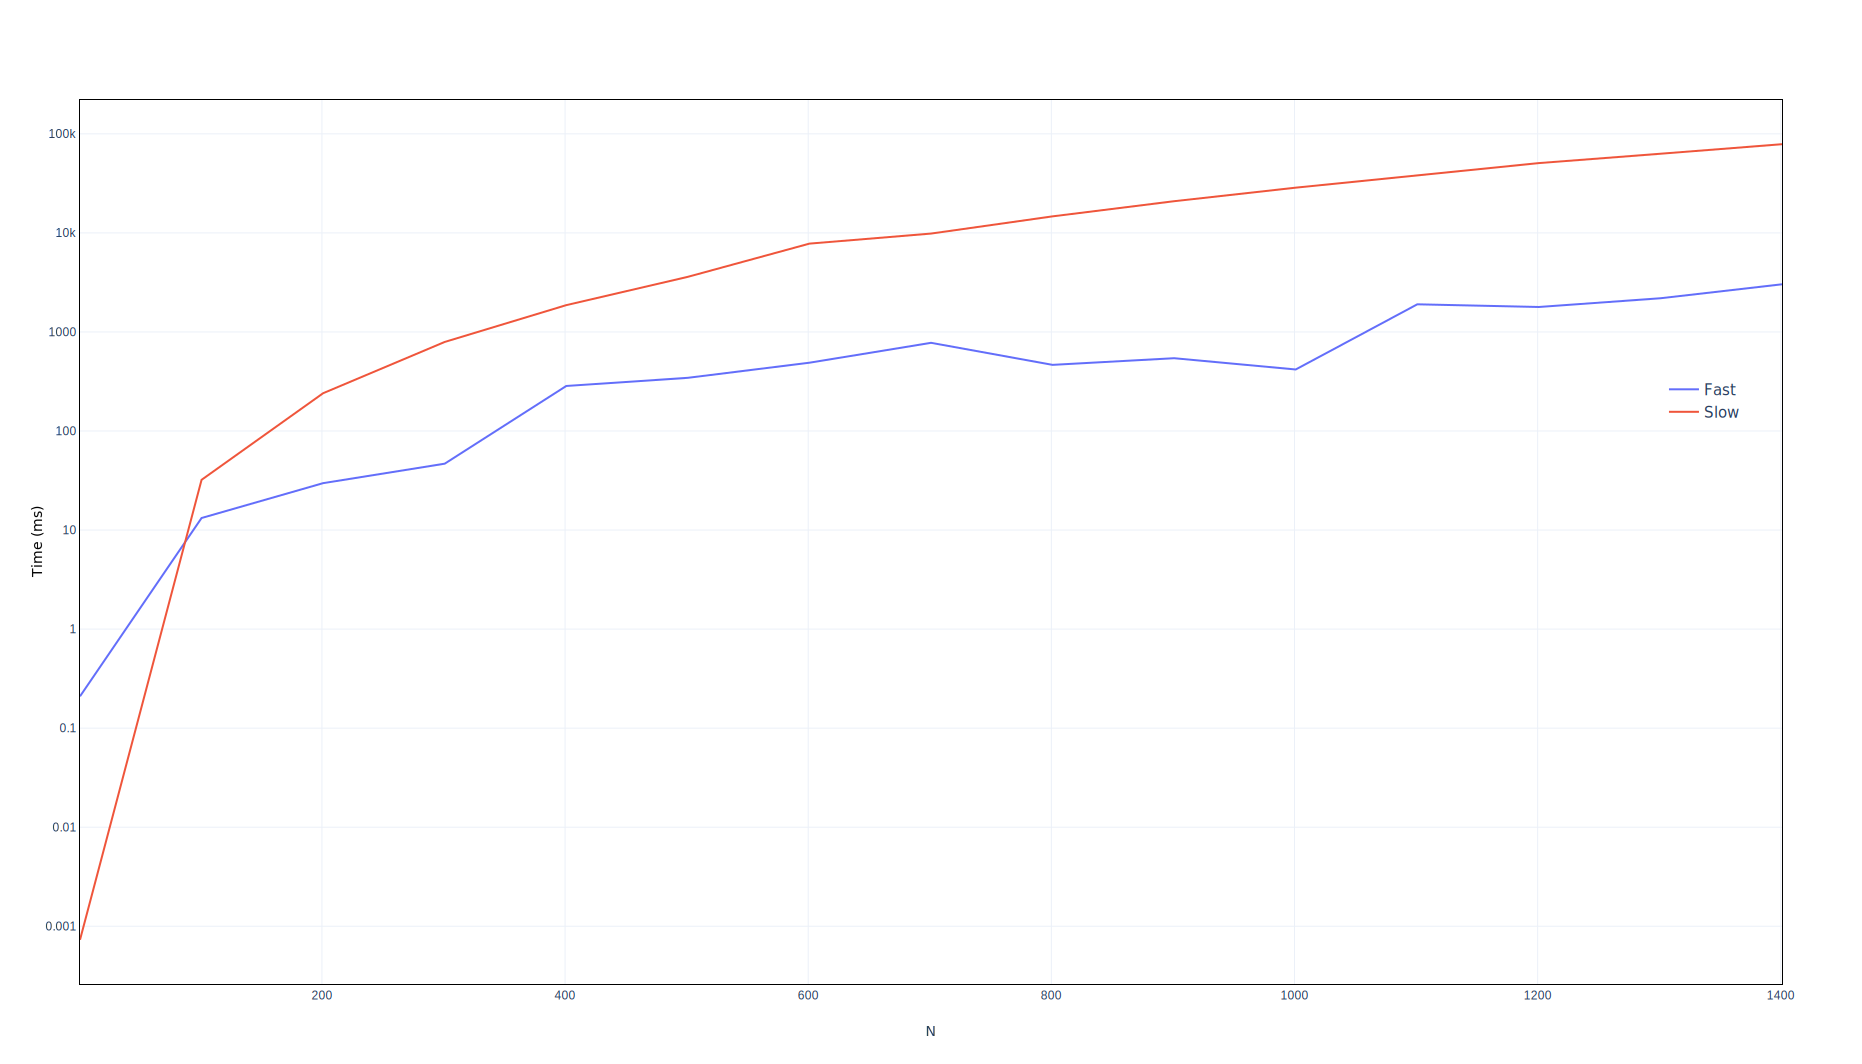
\includegraphics[scale=0.7]{figures/timings}
	\caption{Tempi}
	\label{fig:timings}	
\end{figure}

\FloatBarrier
	

	
	
	
	
	\part{Progettazione di un'interfaccia grafica per la compressione di immagini}
	\FloatBarrier
	\newpage
	\printbibliography
\end{document}
	
